As a comparison point for Pip's ability to manage continuous random variables, we have constructed a sample-first probabilistic extension to Postgres that loosely emulates MCDB's tuple-bundle concept using ordinary Postgres rows.  A sampled variable is represented using an array of floats, while the tuple bundle's presence in each sampled world is represented using a densely packed array of booleans.  In lieu of an optimizer, test queries were constructed by hand so as to minimize the lifespan of either array type.

We evaluated both the Pip C-Tables and the Sample-First infrastructure against three related queries.  Tests were run over a single connection to a modified instance of PostgreSQL 8.3.4 with default settings running on a 2x4 core 2.0 GHz Intel Xeon with a 4MB cache.  All queries were evaluated over a 1 GB database generated by the TPC-H benchmark.  Unless otherwise specified, all sampling processes generate 1000 samples apiece.  Unless otherwise specified, results shown are the average of 10 measurements run sequentially.  

The first set of tests evaluate Pip's performance on queries similar to those used in \cite{MCDB}.  The results of these tests are shown in Figure \ref{fig:querytimings}.  Performance times for Pip are divided into two components: query and sample, to distinguish between time spent evaluating the deterministic components of a query and building the result c-table, and time spent computing expectations and confidences of the results.

\begin{figure}
\begin{center}
\resizebox{3in}{!}{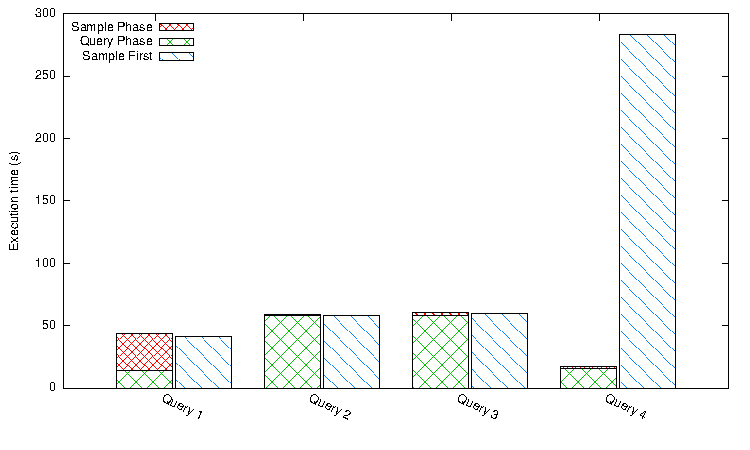
\includegraphics{graphics/query_timings.pdf}}
\caption{Query evaluation times in Pip and Sample-First}
\label{fig:querytimings}
\end{center}
\end{figure}

The first query computes the rate at which customer purchases have increased over the past two years.  The percent increase parametrizes a Poisson distribution that is used to predict how much more each customer will purchase in the coming year.  Given this predicted increase in purchasing, the query estimates the company's increased revenue for the coming year.

In the second and third queries, past orders are used to compute the mean and standard deviation of manufacturing and shipping times.  These values parametrize a pair of Normal distributions that combine to predict delivery dates for each part ordered today from a japanese supplier.  The second query computes the maximum of these dates, while the third compares the times against arbitrary customer satisfaction thresholds to generate a list of potential ``dissatisfied'' customers.

As expected, Pip's performance on these queries is comparable to the sample-first approach.  In the general case, Pip performs effectively the same computations as Sample-First, save that Pip delays sampling slightly longer.  In particular, queries 2 and 3 demonstrate how little time sampling can take for some queries; additional samples can be computed without incurring the nearly 1 minute query time.

The final timing test combines a simplified version of the prior two queries to simulate a risk management query that might be evaluated daily.  Given per-customer revenue forecasts, estimates for product manufacturing and shipping times, customer satisfaction thresholds, compute the expected revenue lost to customers dissatisfied with today's service.  For added realism, this query uses a precomputed table of part production and shipping times (which changes rarely enough that it can be updated monthly).  This query is shown in Figure \ref{fig:timingq4}.

This query includes two distinct, independent sampling components: the expectation of revenue from a customer, and the probability that a customer will be dissatisfied.  A studious user may note this fact and hand optimize the query to compute these values independently.  However, without this optimization, a sample-first approach will generate one pair of values for each customer for each world.  Because worlds where a customer is satisfied are not relevant to the query, an arbitrarilly large number of customer revenue values will be discarded.  Pip separates the computation of expectations and confidences and does not suffer from this problem.  

For this comparison, customer satisfaction thresholds were set such that an average of 10\% of customers were dissatisfied.  Consequently sample-first discarded an average of 10\% of its values.  To maintain comparable accuracies, the sample-first query was evaluated with 10,000 samples while the Pip query remained at 1000 samples.  

\begin{figure}
\begin{center}
\resizebox{3in}{!}{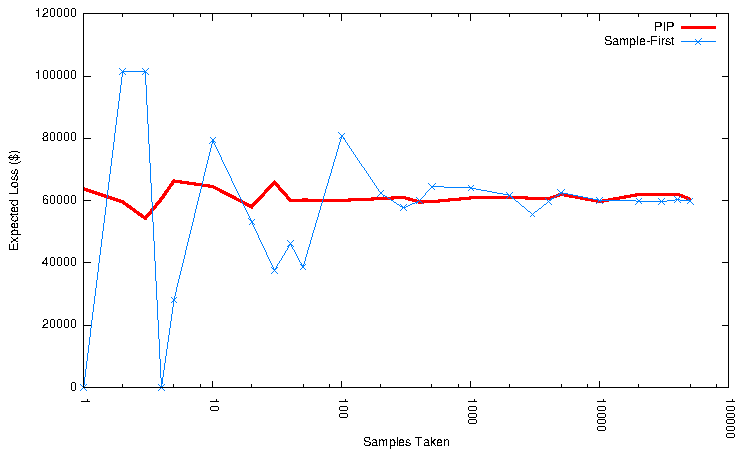
\includegraphics{graphics/iterative_refinement.pdf}}
\caption{Variance as a function of samples in Pip and Sample-First.  Each data point is an estimate generated by a single run at the indicated number of samples}
\label{fig:iterativerefinement}
\end{center}
\end{figure}


Figure \ref{fig:iterativerefinement} demonstrates one extreme case of this in a comparison between Karp-Luby estimates and Sample-First estimates.  The results shown are for repeated executions of a query similar to query 4, save with a filter that removes all but approximately 10 clients.  In queries that do not involve a large linear aggregate, the sample-first approach disqualifies a sufficient number of possible worlds that subsequent expectation computations falter.  Conversely the Karp-Luby estimator has sufficient information that it can employ a precomputed CDF lookup table to compute each row's bag probabilities.  Because of this and the fact that it generates more ``useful'' samples, its results have a much lower variance with far fewer samples required.

We have shown that it is possible to apply the c-tables approach to probabilistic databases with only minimal overhead, even when it is used to represent arbitrary variable distributions.  The additional information provided by the c-table adds a degree of flexibility that allows Pip to outperform Sample-First approaches in a number of instances.

\begin{figure}[t!]
%\footnotesize
\begin{footnotesize}
\begin{verbatim}
create table `shipping_params' as
  select 
    avg   (l_shipdate    - o_orderdate) as ship_mu,
    avg   (l_receiptdate - l_shipdate ) as arrv_mu,
    stddev(l_shipdate    - o_orderdate) as ship_sigma,
    stddev(l_receiptdate - l_shipdate ) as arrv_sigma,
    l_partkey as p_partkey
  from orders,lineitem
  where o_orderkey = l_orderkey
  group by partkey;
alter table params add constraint "p_partkey_pkey" 
  primary key (p_partkey);
-- BEGIN TIMING QUERY --
create temporary table q4_shipping as
  select o_orderkey AS orderkey, o_custkey AS custkey,
    CREATE VARIABLE(`Normal',ship_mu,ship_sigma)
    CREATE VARIABLE(`Normal',arrv_mu,arrv_sigma)
  from  orders,lineitem,shipping_params
  where p_partkey = l_partkey;
   and  o_orderdate = today()
   and  o_orderkey  = l_orderkey;
create temporary table q4_annoyed as
  select custkey from q4_shipping where ship > 120
union all
  select custkey from q4_shipping where arrv > 90;
create temporary table q4_order_increase as
  select o_orderkey, o_custkey,
     CREATE VARIABLE(`Poisson', increase) *
       l_extended_price * (1.0 - l_discount) as rev
  from (select newc / oldc as increase, custkey 
    from (select o_custkey as custkey, 
             sum(o_orderdate.year-1996.0) AS newc,
             sum(1997.0-o_orderdate.year) AS oldc
      where o_orderdate.year = 1997 
        or  o_orderdate.year = 1996
      group by custkey
     ) as counts
   ) as increase_per_cust,
    orders
  where custkey = o_custkey
 ) as var_increase_per_customer,
 (select lineitem.*,
  from  nation,supplier, lineitem, partsupp
  where n_name = 'japan' and n_nationkey = s_nationkey
   and  s_suppkey = ps_suppkey
   and  ps_partkey = l_partkey
   and  ps_suppkey = l_suppkey
 ) as items_from_japan;
-- BEGIN TIMING SAMPLE --
select avg(confidence),
       expected_sum_naive(rev, q4_annoyed)
from   q4_annoyed,
       (select o_custkey as custkey, rev
        from   q4_revenue_gains
       ) as revenues
where  revenues.custkey = q4_annoyed.custkey;
\end{verbatim}
\end{footnotesize}

\vspace{-5mm}

\caption{Timing Query 4}
\label{fig:timingq4}
\end{figure}